\section{Domæneanalyse}

\begin{figure}
	\centering
	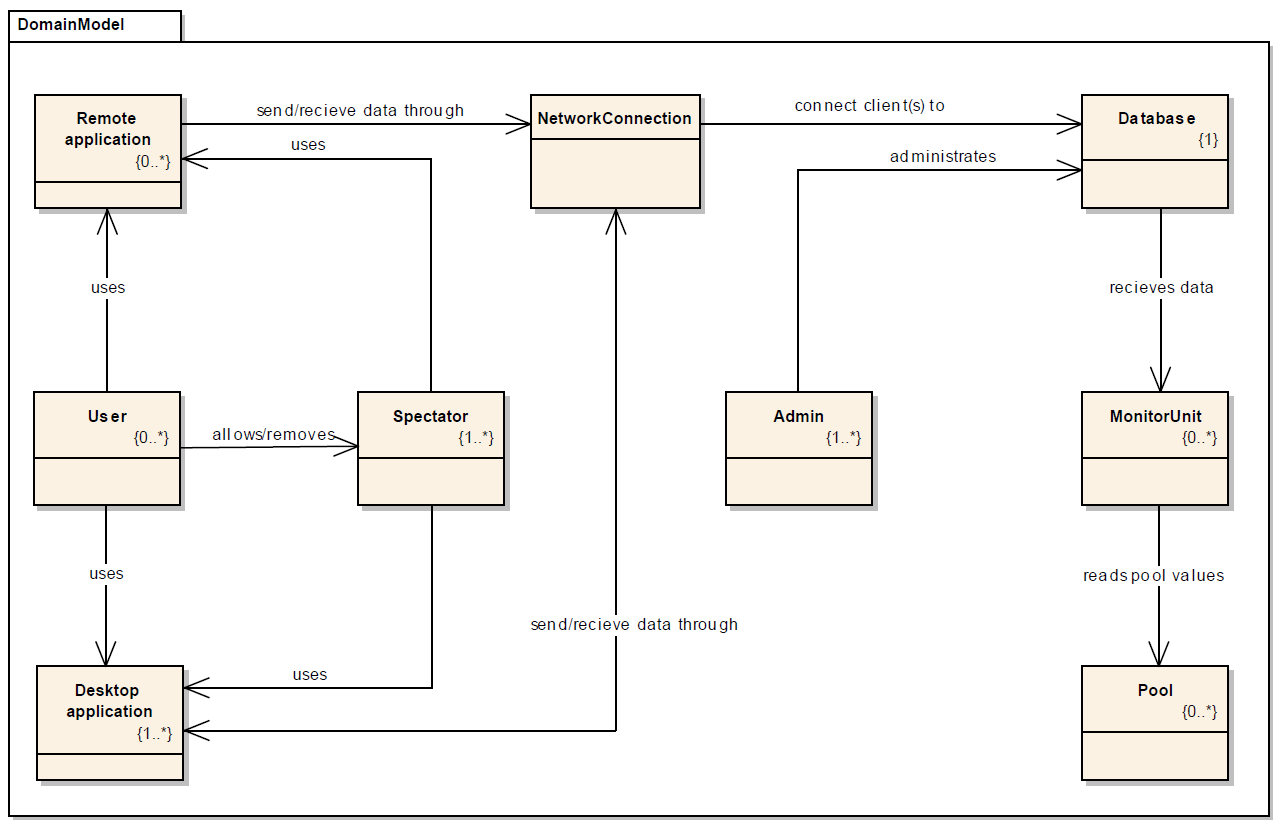
\includegraphics[width=\linewidth]{figs/domainModel}
	\caption{Domænemodel for systemet}
	\label{fig:domainmodel}
\end{figure}

%\todo{Elementer i figur \ref{fig:domainmodel} skal muligvis rykkes tættere sammen for at gøre det nemmere at læse på tryk.}

\subsection{Domænebeskrivelser}
Med udgangspunkt i modellen på figur~\ref{fig:domainmodel} er der opstillet analyser af de enkelte domæner.

\subsubsection{\gls{user}}
\gls{user} er systemet primære bruger. En \gls{user} kan tillade og/eller fjerne \glspl{spectator}. En \gls{user} kan regulere pH/klor/temperatur værdier inden for evt. lovmæssige begrænsninger. Tilføjelse\footnote{Mulighed for tilføjelse af  \gls{mu} giver \gls{user} mulighed for at tilføje flere/større \glspl{pool} og/eller \glspl{mu}.} af \glspl{mu} er \glspl{user} ansvar. En \gls{user} har mulighed for at sende en \gls{specinvite} til en anden \gls{user}. Dette gøres ved at sende et link\footnote{En \gls{user} kan gennem \gls{pcapp} få genereret et link som \gls{user} selv står for at sende.}  til anden partens email-addresse.

\todo{Reference skal muligvis tilføjes.}

\subsubsection{\Gls{spectator}}
En \gls{spectator} er en \gls{user} der med tillladelse fra en anden \gls{user} får mulighed for at se med på dennes pooldata. Hvis den anden \gls{user} har et system bestående af flere \gls{mu}.

\subsubsection{\gls{pcapp}}
\gls{pcapp} primære formål er at gengive pooldata som findes på Databasen. En \gls{user} kan igennem \gls{pcapp}:

\begin{itemize}
	\item Logge ind med personlig brugerprofil.
	\item Generere et link til invitation af \gls{spectator}.
	\item Se grafisk gengivelse af historisk data.
	\item Se nuværende Pool data.
	\item Sætte \gls{tv} for Pool.
	\item Registrere en eller flere \gls{mu}.
\end{itemize}

\subsubsection{\gls{iosapp}}
En \gls{iosapp} er en “lightweight” udgave af \gls{pcapp}. Denne applikations formål er at \gls{user} kan danne sig et overblik over dataen fra de \gls{mu} der er tilknyttet konto.

\subsubsection{NetworkConnection}
Til at transmittere data fra \gls{mu} til Database, samt fra Database til \gls{pcapp} og \gls{iosapp} benyttes en netværksforbindelse.  For at systemet skal fungere er det et krav at både \gls{pcapp} og remote applikation, databaseserver samt \gls{mu}\footnote{  \gls{mu} har ikke en direkte forbindelse til internettet, men benytter sig af en endnu ikke defineret mediator.} har forbindelse til internettet.

\subsubsection{\gls{admin}}
En \gls{admin} er en “official” fra \gls{smartpool}, og har rettigheder til at fjerne brugere fra systemet. Det er \glspl{admin} ansvar at de lovmæssige standarder%\todo{Reference} for pH/klor/varme værdier er defineret i Databasen.

\subsubsection{\gls{db}}
Databasen indeholder brugerdata, såsom brugerens email-adresse, registrerede \gls{mu}, samt måledata. Måledata gemmes i en endnu udefineret tidsperiode, således at \gls{user} har mulighed for at få en grafisk gengivelse\footnote{Evt. Graf, søjlediagram og lign.} af historisk data.

\subsubsection{\gls{mu}}
En \gls{mu} registreres hos \gls{smartpool} gennem \gls{pcapp} applikationen. Med hver \gls{mu} medfølger et serienummer som bruges ved registrering. En \gls{mu} er enheden der måler pH, frit\footnote{Frit klor angriber bakterier, alger og svampeorganismer. Med tiden transformeres frit klor til bunden klor.} klor og total\footnote{Total klor er summen af frit klor og bunden klor.} klor samt varmeværdier i en \gls{pool}. Det er \gls{mu} der står for behandling\footnote{Da der er en sammenhæng~\ref{fig:chlorinePh} mellem målte pH-værdier og effektivitet af frit klor skal den rå data gennemgå en hidtil udefineret matematisk behandling for at kunne vise \gls{user} relevant information.} af rå data. De rå data bruges til at beregne forholdet mellem bunden\footnote{Bunden klor er ineffektivt, lugter kraftigt og irriterer øjne og slimhinder.} klor og frit klor samt \glspl{pool} overordnede sundhedskarakteristika. \gls{mu} ansvar er således:

\todo{Reference}
\todo{Reference.}
\todo{Reference.}

\paragraph{Måling af data}
\begin{itemize}
	\item Måling af total klor.
	\item Måling frit klor.
	\item Måling af pH-værdi.
	\item Måling af Temperatur.
\end{itemize}

\paragraph{Behandling af rå data}
\begin{itemize}
	\item Beregning af bunden klor.
	\item Beregning af klor der bør tilføres/fjernes fra \gls{pool}.
	\item Beregning af den mængde syre/base der skal tilføres \gls{pool}.
\end{itemize}

\begin{figure}
	\centering
	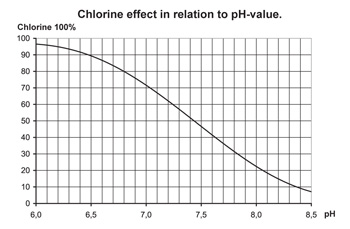
\includegraphics[width=0.6\linewidth]{figs/chlorinePh.png}
	\caption{Sammenhæng mellem effektivitet af frit klor og pH værdi. Kilde: \url{http://www.pahlen.com/users-guide/ph-and-chlorine}}
	\label{fig:chlorinePh}
\end{figure}


\subsubsection{\gls{pool}}
Pool er den enhed der males på. En Pool kan være af hvilken som helst størrelse og form. Hver Pool kan associeres med en \gls{mu}.